\documentclass[11pt]{article}

\usepackage[letterpaper,margin=1in]{geometry}
\usepackage{amsmath,amssymb}
\usepackage{booktabs}
\usepackage{microtype}
\usepackage{times}
\usepackage[T1]{fontenc}
\usepackage[utf8]{inputenc}
\usepackage{titlesec}
\usepackage[hidelinks]{hyperref}
\usepackage{url}
\Urlmuskip=0mu plus 1mu\relax
\usepackage{xcolor}
\usepackage{graphicx}
\graphicspath{{figs/}}

\titleformat{\section}{\normalfont\large\bfseries}{\thesection}{0.6em}{}
\titleformat{\subsection}{\normalfont\normalsize\bfseries}{\thesubsection}{0.5em}{}
\setlength{\parskip}{0.4em}
\setlength{\parindent}{0pt}
\renewcommand{\arraystretch}{1.15}

\title{\textbf{What Aggregation Does to Epistemic Content:\\ A Behavioral
Characterization of Multi-Seat LLM Pipelines}}
\author{Sam Bobo}
\date{Draft v0.1 --- August 2026 \quad$\vert$\quad Target: arXiv cs.CL}

\begin{document}
\sloppy
\maketitle

\begin{abstract}
\noindent
Multi-seat pipelines route a question to several specialist models and combine
their answers with a final model. We characterize what that final step does to
the epistemic content it receives---the labelled assumptions, jurisdictional
distinctions, and disclosures of uncertainty the specialists write---by
tracking each such marker from the seat that raised it to the finished answer,
across roughly 1{,}400 audited runs on a single consumer machine.

The aggregation step is not a channel. Of the behavior families the specialists
raise, it preserves about $72\%$ and discards the rest at a rate that does not
depend on how much arrives. It also \emph{invents}: on questions where the
specialists raise little, more than a third of what the final answer contains
traces to no specialist at all, against a ninth on questions where they raise
plenty. The step therefore writes toward a characteristic level, preserving
faithfully when supplied and manufacturing content when starved, and a
$2.6\times$ distinction the specialists draw between demanding and undemanding
questions reaches the page as $1.8\times$. Around that behavior we map what the
step responds to and what leaves it unmoved. It responds to its own
instructions, gradedly and with per-behavior specificity: output rises with the
number of preservation clauses, and each clause moves exactly the behavior it
names and no other. It is close to invariant under everything upstream---the
volume of qualification the specialists produce (raising it lowers the output,
monotonically), the number of specialists, the pipeline topology, and
weight-level training at either end under three optimizers and two reward
designs. We report these as measured regularities of the aggregation step
rather than as an argument for or against building such pipelines.
\end{abstract}

\section{Introduction}
A multi-seat pipeline is a system with a distinguished component. Several
models contribute, but one of them writes the text a user reads, and whatever
the others produced reaches the user only through that final act of writing.
This paper is about the behavior of that step.

We study it on one kind of content: \emph{epistemic} markers---a number
labelled as an assumption rather than a fact, a distinction drawn between two
regulatory regimes, a note that some figure may have changed since the model
was trained, a calibrated hedge. This content is a good probe for two reasons.
It is identifiable in text, so it can be traced from where it was written to
where it ends up. And it is the kind of content that matters most when it goes
missing: a confident synthesis of hedged inputs misrepresents what the system
actually knows.

Our question is descriptive. Given that a specialist wrote a caveat, what
happens to it? Given that the specialists collectively wrote more or fewer
caveats, what happens to the total? What changes the answer, and what does
not?

We report three groups of findings. Section~\ref{sec:prov} follows individual
behavior families through the aggregation step and decomposes the output into
what was preserved, what was discarded, and what was invented.
Section~\ref{sec:resp} characterizes the one input the step responds to
strongly---its own instructions---including how gradedly and how specifically.
Section~\ref{sec:inv} reports the manipulations that leave it essentially
unmoved, which is the larger set. Section~\ref{sec:model} assembles these into
a compact behavioral description.

We are describing one instantiation of a common pattern, not proving a
theorem, and Section~\ref{sec:limits} is explicit about what that licenses.

\section{Apparatus and measurement}
\textbf{Pipeline.} A planner decomposes the question and dispatches a
self-contained sub-question to each relevant specialist; specialists never see
the original query. A final model then writes the answer from their
contributions under an instruction that asks it to surface disagreements and
to preserve specific things the specialists flagged (Appendix~\ref{app:prompt}).
Four open-weights models at or below 20B run locally on one 32\,GB machine:
Phi-4-14B as planner and writer unless stated, with Llama3-Med42-8B,
Saul-7B-Instruct and Qwen-Open-Finance-8B as specialists. Variants substitute
gpt-oss-20B or Qwen2.5-7B in the writing role.

\textbf{What we count.} Four families of epistemic behavior: disclosure that
information may post-date training, labelling a quantity as an assumption,
distinguishing jurisdictions or regimes, and calibrated hedging. A fifth we
defined---distinguishing near-synonymous terms of art---fell below detection on
two independent instruments and is dropped. We report both the \emph{density}
of markers per thousand characters and, where provenance matters, the number of
distinct families present, which is insensitive to repetition.

\textbf{Provenance.} Because each specialist's contribution appears verbatim in
the writing model's prompt, we can determine for any finished answer which
families were \emph{raised} upstream, which of those were \emph{preserved},
and which appear in the output having been raised by nobody. This is the
measurement the paper rests on and it requires no additional model calls.

\textbf{Instruments.} Pattern matching is primary. Every load-bearing
comparison is re-scored by a calibrated entailment model and by blinded
pairwise LLM judges shown both texts in each order and required to quote their
evidence. Where the three disagree we say so; one finding produced by pattern
matching alone did not survive and was retired (Appendix~\ref{app:instr}).

\textbf{Scale.} Roughly 1{,}400 runs, five seeds per condition, bootstrap
intervals throughout. Predictions were registered before the runs that test
them, including several that failed.

\section{What the step preserves, discards, and invents}
\label{sec:prov}

\begin{figure}[t]
\centering
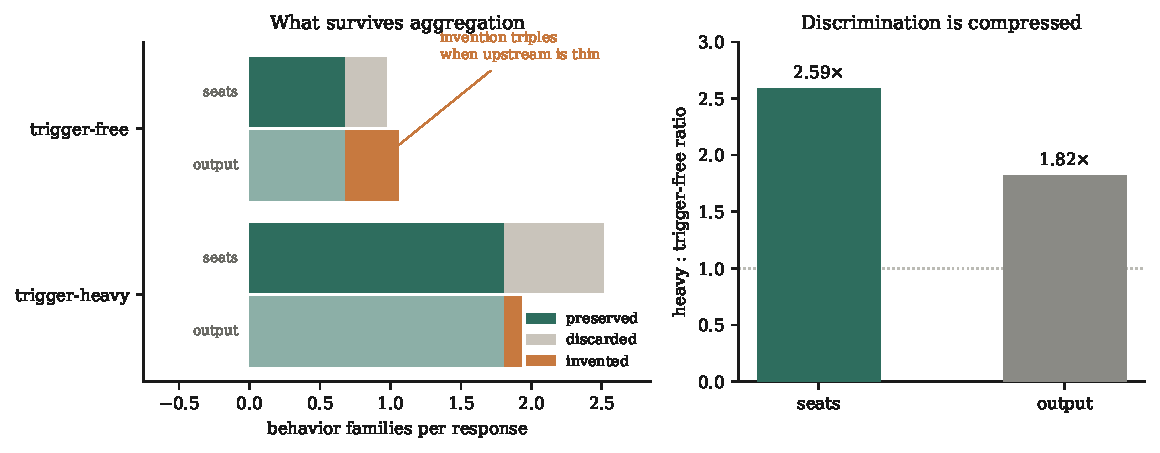
\includegraphics[width=\linewidth]{fig_provenance.pdf}
\caption{\emph{Left:} for each condition, the upper bar is what the
specialists raised, split into preserved and discarded; the lower bar is what
the finished answer contains, split into traceable and invented.
\emph{Right:} the ratio between demanding and undemanding questions, as the
specialists draw it and as it reaches the page. Means over 648 syntheses.}
\label{fig:prov}
\end{figure}

\begin{table}[t]
\centering
\caption{Provenance of behavior families, per response (648 syntheses).}
\label{tab:prov}
\begin{tabular}{lccccc}
\toprule
Question type & raised & preserved & discarded & invented & traceable \\
\midrule
trigger-heavy & $2.51$ & $1.81$ & $0.70$ & $0.12$ & $94\%$ \\
trigger-free & $0.97$ & $0.68$ & $0.29$ & $\mathbf{0.38}$ & $\mathbf{64\%}$ \\
\bottomrule
\end{tabular}
\end{table}

Three regularities appear in Table~\ref{tab:prov}.

\textbf{Discard is proportional.} The step drops $28\%$ of raised families on
demanding questions and $30\%$ on undemanding ones. Loss is close to a
constant fraction of what arrives rather than a fixed amount, and does not
depend on how much is supplied.

\textbf{Invention is not proportional---it compensates.} On demanding
questions almost nothing in the output is untraceable ($0.12$ families,
$94\%$ traceable). On undemanding questions, where the specialists raise
little, invention more than triples in absolute terms and over a third of the
output traces to no specialist. The step is not simply lossy; when the supply
of genuine qualification is thin, it produces qualification anyway.

\textbf{Distinctions compress.} The specialists draw a $2.59\times$ distinction
between demanding and undemanding questions ($2.51$ families against $0.97$).
What reaches the page is $1.82\times$ ($1.94$ against $1.06$). Loss at the top
and invention at the bottom together compress the distinction the upstream
models drew. The information that a question warranted little caution is
available in the pipeline and is substantially attenuated by the time it is
written.

A convenient summary is that the writing step behaves as though it has a
target level of epistemic content. Given more than that, it trims; given
less, it fills. The following two sections test that description against the
step's response to interventions.

\section{What the step responds to}
\label{sec:resp}
One intervention moves the aggregation step substantially: the instructions
given to it.

\begin{figure}[t]
\centering

\includegraphics[width=\linewidth]{fig_gain.pdf}
\caption{\emph{Left:} output rises with the number of preservation clauses
retained in the writing model's instructions, on three different writers.
\emph{Right:} giving the same disposition instruction to more specialists
leaves the output flat to declining.}
\label{fig:gain}
\end{figure}

\textbf{The response is graded, not switch-like.} Retaining $k \in
\{0,1,2,3\}$ preservation clauses raises output on all three writers tested
(Spearman $\rho = +1.00$, $+0.80$, $+0.80$), spanning $2$--$3\times$ on two of
them and $1.3\times$ on the third. The relationship is a monotone trend rather
than strict monotonicity: only one writer increases at every step, with the
other two showing a single-cell dip within the noise of six observations per
point. Holding the pipeline, the models, and the specialists' text fixed and
changing only these clauses moves output from $0.159$ to $0.525$ on one writer
and $0.575$ to $1.211$ on another.

\textbf{The response is specific to the behavior named.} Isolating clauses one
at a time shows each moving exactly the family it names and leaving the others
flat: the numeric-framing clause raises labelled assumptions from $0.003$ to
$0.499$; the caveats clause raises cutoff disclosure from $0.000$ to $0.035$;
the vocabulary clause raises its own family from $0.000$ to $0.014$. These are
targeted specifications rather than general encouragement to be careful, which
rules out the alternative that instructions simply put the writer in a more
cautious mood.

\textbf{Aggregate movement goes to whichever clause matches the writer's
profile.} Under one writer, the numeric clause alone accounts for $126\%$ of
the full block's effect while the others land on baseline---not because they
fail, but because the behaviors they name are ones this writer barely produces
in the first place. Which behavior dominates differs by writer: cutoff
disclosure accounts for most of the composite under two writers ($0.554$,
$0.909$) and almost none under a third ($0.018$). Any recommendation about
which clause to write is therefore conditional on the writer.

\textbf{Clauses interfere mildly.} Single-clause effects sum to $+0.41$
against the assembled block's $+0.35$, and the strongest single clause alone
slightly exceeds the full block. Adding clauses aimed at behaviors a writer
does not produce appears to compete with the one that works.

\section{What leaves the step unmoved}
\label{sec:inv}
The larger set of findings is negative in form and, we think, more informative
for it: these are the invariances that constrain what a behavioral account can
look like.

\textbf{Invariant under upstream volume---and inversely responsive.} Raising
what the specialists produce does not raise the output. Prompting a specialist
to qualify more doubles what it writes ($0.84 \rightarrow 1.82$) while the
finished answer falls ($1.21 \rightarrow 0.92$); training it on
qualification-rich examples reproduces this ($1.75$ at the seat, $0.92$ at the
mouth). Extending the treatment to more specialists lowers the output
monotonically, from $1.01$ at none to $0.64$ at all three ($\rho = -0.80$).
Over-dense input does not merely fail to transmit; on one writer it inverts,
$1.17 \rightarrow 0.61$.

\textbf{Invariant under the number of demands.} Constructing questions that
demand one, two, three, or four distinct kinds of qualification, with length
held constant, leaves the output flat ($\rho = +0.20$, non-monotone, $L{=}4$
overlapping $L{=}1$). Across the same range the writer engages $1.2$--$1.7$
families regardless of how many were asked for. Between-question variance at
fixed demand exceeds any variation across demand.

\textbf{Invariant under topology.} Holding the model fixed in every role and
varying only the arrangement, three specialists merged plainly reach $0.16$
against a single model's $0.14$; two full rounds of debate reach $0.16$; a
single model that drafts, critiques itself and revises reaches $0.08$. A
single model given a good instruction and no specialists at all reaches $0.50$,
against the full pipeline's $0.57$, intervals overlapping.

\textbf{Invariant under weight-level training, at both ends.} Reference-free
preference optimization on a specialist installs no additional qualification
($0.85$ against $0.84$ untrained) and tripling the training data changes
nothing, though the larger corpus raised the model's own accuracy at
distinguishing good examples from bad from $0.48$ to $0.94$. Replication on a
second specialist of a different lineage produced no effect; on a third, an
effect registered in advance failed to appear. Training the \emph{writing}
model directly leaves its output where it started ($0.89$ against $1.03$), and
so does an on-policy retry whose reward was computed on the finished answer and
shaped to reward qualification where warranted and penalize it where not
($0.60$ against $0.56$). Notably, after training the writer on precisely the
behavior its instructions elicit, those instructions still worked at full
strength ($1.58\times$ against an untrained $1.82\times$), which suggests the
two act on different things.

\textbf{Not invariant under choice of writer.} Substituting the model in the
writing role changes the output under identical input, which is the one
structural change that does move it.


\section{The one output with no single-model analogue}
\label{sec:tension}
Everything measured so far concerns how much epistemic content the step emits,
and on that axis a well-instructed single model matches the pipeline. There is
one output where no such comparison is possible.

The writing instruction asks, before the answer is drafted, for an explicit
enumeration of tensions between the specialists---places where following one
contribution makes another harder. This is the only part of the pipeline's
output that a single model cannot produce by construction: identifying a
conflict requires more than one source to conflict.

\begin{table}[t]
\centering
\caption{Tension enumeration by arrangement. Only arrangements with a genuine
aggregation step produce one.}
\label{tab:tension}
\begin{tabular}{lccc}
\toprule
Arrangement & runs & responses with a tensions section & tensions per response \\
\midrule
council (all variants) & $195$ & $86$--$100\%$ & $3.0$--$3.9$ \\
flat merge & $50$ & $0\%$ & $0.00$ \\
single model $+$ instruction & $90$ & $0\%$ & $0.00$ \\
\bottomrule
\end{tabular}
\end{table}

The separation is categorical rather than a matter of degree
(Table~\ref{tab:tension}). Arrangements that pass specialist text to a writer
without asking for tensions produce none at all; the council produces close to
four per response, reliably.

\textbf{Are they grounded?} Given the invention behavior of
\S\ref{sec:prov}, the obvious concern is that these conflicts are
manufactured. Many tensions cite a specific figure and attribute it to a named
specialist, which makes them checkable: the figure either appears in that
specialist's contribution or it does not. Across $210$ such tensions,
$\mathbf{89\%}$ cite a figure that is genuinely present upstream (median
$100\%$ per response); $11\%$ cite one that appears nowhere.

This is a notably better rate than the step's handling of epistemic content on
thin questions, where $36\%$ of what it emits is untraceable. The step
invents caveats far more readily than it invents disagreements---which are
different behaviors, and the asymmetry is the more interesting result.

\textbf{An extension that failed, and why it is worth reporting.} The $89\%$
covers only tensions citing a figure. We attempted to extend the check to the
$139$ qualitative ones using the entailment instrument that validates our
other measurements, and it does not transfer. On the figure-citing subset
where both methods apply, entailment scores $16\%$ grounded against
figure-matching's $89\%$, and the two agree on only $23\%$ of items.
Decomposing each tension into its component claims---a tension is typically a
compound contrastive statement, ``A recommends $x$, but B assumes
$y$''---raises the entailment rate to $48\%$ with at least one clause
supported, and the median best-clause entailment sits at $0.57$, just under
our $0.60$ threshold.

The diagnosis is that entailment is the wrong relation here. A tension clause
is a \emph{paraphrased summary} of what a specialist wrote, not a restatement
of it, and no single upstream sentence entails a claim that combines two
contributions with a conflict framing. What the instrument measures on this
material is paraphrase distance rather than groundedness, which is why its
scores cluster at the decision boundary. We therefore report the figure-based
result, which is unambiguous, and record the qualitative majority as not
measurable by the instruments we have. Establishing it would need human
judgement or a judge shown both contributions and asked whether the conflict
is real.

This is the third occasion in this work on which an instrument disagreed with
another and the disagreement, rather than either number, was the finding.

\section{A behavioral description}
\label{sec:model}
The regularities above are compactly summarized as follows. The aggregation
step behaves like a writer with a target level of epistemic content rather
than a channel that conveys it. That target is set by the step's instructions,
gradedly and per-behavior, and modulated by which model occupies the role.
Content arriving from upstream is preserved at a roughly constant rate when it
is plentiful and supplemented by invention when it is scarce, with the
consequence that distinctions drawn upstream reach the output attenuated.

Two predictions follow that we did not set out to test but that the data
support. First, interventions that increase upstream qualification should be
counterproductive, because they push past the target and the excess is
trimmed---which is what the seat-tuning and multiple-specialist results show.
Second, a system's apparent indifference to input should be strongest where
input is thinnest, because that is where invention is doing the most work---
which is what the $94\%$ against $64\%$ traceability split shows.

The description also has a boundary. It concerns epistemic content that
passes \emph{through} the step. The tension enumeration of
\S\ref{sec:tension} is content the step \emph{constructs}, and it behaves
differently: it is far more faithful to upstream ($89\%$ of checkable
tensions grounded) than the step's handling of caveats on thin input ($64\%$
traceable). Whatever produces compensating invention does not operate on
constructed conflicts to the same degree.

One thing this description does not explain is why instructions move the step
when weight-level training does not. Three accounts are consistent with our
data---that the capability is present and instructions retrieve rather than
install it; that the target behavior is conditional on information available
only at inference; and that training and instructing act on different
mechanisms, as the surviving instruction effect after training suggests---but
we cannot distinguish among them, and our training was small enough that scale
remains a live alternative.

\section{Limitations}
\label{sec:limits}
Of five behavior families we set out to track, one fell below detection on
both instruments, so we report four; the instruction effect is clear on the
combined measure but not on any single behavior alone. Pattern matching misses
paraphrase and rewards brevity, and although two further instruments agree
with it on the load-bearing comparisons, all three are automatic and none is
anchored to human judgement.

Everything ran at or below 20B parameters on one consumer machine, with five
seeds and seven questions we wrote ourselves plus eleven added for specific
tests. A frontier model in the writing role could behave differently. The
topology comparison uses one model family throughout and one implementation of
each arrangement. Full policy-gradient reinforcement learning could not be
attempted: on a 34\,GB machine, group-relative optimization of a 7B writer with
$2.2$k-token prompts and a $152$k vocabulary exhausts memory before the first
update, so the invariance under training is established for offline preference
optimization and an on-policy best-of-$n$ surrogate only.

We report defects in our own record rather than repairing them. One model
intended for a lineage comparison produced degenerate output---26 of 30
answers were fragments ending mid-sentence---and that arm is withdrawn, taking
the comparison with it. A claim about the pipeline's behavior on undemanding
questions was found, after publication of a figure computed from it, to have
been measured on runs where the planner consulted no specialists and the
writing instruction was consequently never applied; those runs were relabelled
and the comparison rerun on questions the planner does engage with. In our
earliest arms, five runs per question are one run from an earlier session plus
four from a later one, and 133 runs record a batch label where a model
identifier belongs.

\section{Implications}
For practitioners the description above has direct consequences. Effort spent
making upstream components more epistemically careful is not merely wasted but
counterproductive at the output. Effort spent on the writing model's
instructions is the intervention with measured, graded effect, and should be
written for the behaviors that writer actually produces. Systems should be
evaluated on questions that warrant no qualification as well as those that
do, since the invention behavior is invisible otherwise.

For the study of such systems, the finding we would most like to see tested
elsewhere is compensating invention. If it generalizes, then a pipeline's
apparent robustness---output that changes little as inputs vary---is partly an
artifact of the aggregation step filling gaps, and evaluations that measure
only what the output contains, without asking where it came from, will
systematically overstate how much of it is grounded.

\paragraph{Reproducibility.} Code, prompts, all runs, pre-registrations,
protocol amendments, refuted predictions, and integrity audits:
\url{https://github.com/srbobo/council-of-experts-research}.

\appendix

\section{The writing model's instruction}
\label{app:prompt}
Two steps: identify tensions between the specialists, then write the
integrated answer. The second step carries five requirements, of which three
are preservation clauses. Verbatim:

\begin{quote}\small
\textbf{1.} Acknowledge the tensions you just identified---not abstractly, but
at the points where they bite the answer.

\textbf{2. PRESERVE numeric framing}---if a specialist labeled a number as a
modeled assumption, your synthesis MUST also label it as an assumption (use
``modeled at,'' ``assumed''). Never adopt a specialist's modeled number as a
fact.

\textbf{3. PRESERVE precise vocabulary}---if a specialist used a specific legal
term, jurisdiction, FDA pathway, or clinical concept, preserve it; do not
smooth out precision in the name of accessibility.

\textbf{4. PRESERVE caveats}---if a specialist flagged training-cutoff
uncertainty or data fragility, propagate that flag into your synthesis.

\textbf{5.} Use whatever structure best fits the user's question.
\end{quote}

Clauses 2--4 are conditional on something a specialist did; clause 1 is not,
and tested alone it changes nothing. Note that the block specifies what to
preserve and never what not to add, which is consistent with the invention
behavior of \S\ref{sec:prov}.

\section{Instruments}
\label{app:instr}
Pattern matching over four families is primary. An entailment model calibrated
against construction-labelled pairs and blinded pairwise LLM judges, shown both
texts in each order and required to quote evidence, check every load-bearing
comparison. One finding did not survive: an apparent \emph{increase} in
hedging on one specialist appeared under pattern matching alone and neither
other instrument saw it. We retired it as an artifact of the measure.

\end{document}
